56. Решим данное уравнение графически. Правая часть представляет из себя гиперболу, а левая --- модуль, коэффициент при котором влияет на то, насколько большой угол при вершине $(5;0)$ будет образован.
$$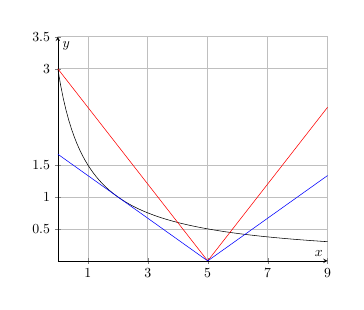
\begin{tikzpicture}[scale=0.5]
\begin{axis}[
    axis lines = middle,
    grid=major,
    legend pos={south west},
    xlabel = {$x$},
    %xlabel style={below right},
    ylabel = {$y$},
    ymax=3.5,
    xtick={1, 3, 5, 7, 9},
    xticklabels={1, 3, 5, 7, 9},
    ytick={0.5,1,1.5,3,3.5},
    yticklabels={0.5,1,1.5,3,3.5},
               ]
	\addplot[domain=0:9, samples=100, color=black] {3/(x+1)};
    \addplot[domain=0:9, samples=100, color=red] {0.6*abs(x-5)};
    \addplot[domain=0:9, samples=100, color=blue] {abs(x-5)/3};
	%\addlegendentry{$\text{Рис. 1}$};
\end{axis}
\end{tikzpicture}$$
Чем больше значение $a,$ тем меньше угол и, соответственно, выше точка пересечения с осью ординат. Гипербола пересекает её при $y=\cfrac{3}{0+1}=3.$ Найдём, при каком значении $a$ график модуля также пройдёт через эту точку: $a\cdot|0+1|=3,\ a=\cfrac{3}{5}.$ При $a>\cfrac{3}{5}$ гипербола будет иметь с модулем ровно две точки пересечения. При $a\leqslant\cfrac{3}{5}$ они будут иметь сначала 3 точки пересечения, затем 2 (в случае касания), затем 0. Найдём, при каком значении $a$ график модуля касается гиперболы. Это происходит при $x<5,$ значит уравнение $a\cdot(5-x)\cfrac{3}{x+1}$ должно иметь единственное решение, то есть $a(5-x)(x+1)=3,\
5ax+5a-ax^2-ax=3,\ ax^2-4ax+3-5a=0$ имеет единственное решение. При $a=0$ точек пересечения нет, значит $\cfrac{D}{4}=4a^2-3a+5a^2=9a\left(a-\cfrac{1}{3}
ight)=0,$
откуда $a=\cfrac{1}{3}.$ Итого ответом является множество $\left\{\cfrac{1}{3}
ight\}\cup\left(\cfrac{3}{5};+\infty
ight).$\\
